\documentclass[11pt]{article}


\usepackage[left=1in, right=1in, top=1in, bottom=1in]{geometry}
\usepackage{amsmath}
\usepackage{amsfonts}
\usepackage{graphicx}
\usepackage{listings}
\usepackage{color}
\usepackage{float}
\usepackage{caption}
\usepackage{subcaption}
\usepackage{fancyhdr}
\usepackage{pgfplots}
\usepackage{algorithm}
\usepackage{algpseudocode}
\usepackage{placeins}
\usepackage{tikz}
\usetikzlibrary{arrows.meta, positioning, calc}
\pgfplotsset{compat=1.18}

\title{Blocked Dynamic Sparse Attention}
\author{Mehul Goel (mehulg), Saransh Agrawal (saransh2) \\ \small Website: https://mehulgoel873.github.io/15418-final-project/}
\date{}

\thispagestyle{plain}
\pagestyle{fancy}
\fancyhf{}
\lhead{Blocked Dynamic Sparse Attention}
\rhead{Mehul Goel, Saransh Agrawal}
\setlength{\headheight}{14pt}

\begin{document}
\maketitle

\section*{Summary}
We are going to implement optimized versions of attention blocks for machine learning applications on the NVIDIA GPUs in the lab. We want to compare a variety of implementations on training speed, accuracy, and perform a detailed analysis of the characteristics of each algorithm. 


\section*{Background}

The core computation in transformer-based models is the \textit{scaled dot-product attention} mechanism, defined as:
\[
\text{Attention}(Q, K, V) = \text{softmax}\!\left(\frac{QK^T}{\sqrt{d_k}}\right) V
\]
where $Q, K, V \in \mathbb{R}^{n \times d_k}$ are the query, key, and value matrices derived from input embeddings, $n$ is the sequence length, and $d_k$ is the head dimension. The diagram below illustrates the dataflow of this computation:

\begin{figure}[H]
\centering
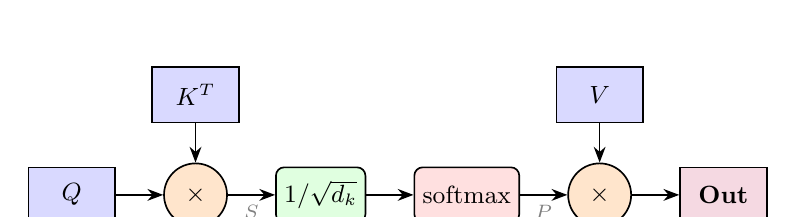
\begin{tikzpicture}[
    node distance=0.7cm,
    input/.style={rectangle, draw, fill=blue!15, minimum width=1.1cm, minimum height=0.7cm, align=center, font=\small\bfseries, inner sep=3pt},
    matmul/.style={circle, draw, fill=orange!20, minimum size=0.8cm, align=center, font=\small\bfseries, inner sep=2pt},
    op/.style={rectangle, draw, rounded corners=3pt, fill=green!12, minimum height=0.7cm, align=center, font=\small, inner sep=3pt},
    output/.style={rectangle, draw, fill=purple!15, minimum width=1.1cm, minimum height=0.7cm, align=center, font=\small\bfseries, inner sep=3pt},
    ->, >=Stealth, semithick
]
    % Main horizontal chain
    \node[input] (Q) {$Q$};
    \node[matmul, right=0.6cm of Q] (mm1) {$\times$};
    \node[op, right=0.6cm of mm1] (scale) {$1/\sqrt{d_k}$};
    \node[op, right=0.6cm of scale, fill=red!12] (sm) {softmax};
    \node[matmul, right=0.6cm of sm] (mm2) {$\times$};
    \node[output, right=0.6cm of mm2] (out) {Out};

    % K feeds into first matmul from above
    \node[input, above=0.5cm of mm1] (K) {$K^T$};
    % V feeds into second matmul from above
    \node[input, above=0.5cm of mm2] (V) {$V$};

    % Edges
    \draw (Q) -- (mm1);
    \draw (K) -- (mm1);
    \draw (mm1) -- node[below, font=\scriptsize, text=gray]{$S$} (scale);
    \draw (scale) -- (sm);
    \draw (sm) -- node[below, font=\scriptsize, text=gray]{$P$} (mm2);
    \draw (V) -- (mm2);
    \draw (mm2) -- (out);
\end{tikzpicture}
\caption{Dataflow of scaled dot-product attention.}
\end{figure}

This computation involves two matrix multiplications ($QK^T$ and the product with $V$) separated by an element-wise scaling and a row-wise softmax. While the matrix multiplications are straightforward to parallelize on NVIDIA GPUs---each output element can be computed independently---the softmax operation introduces a key challenge.

The softmax function, $\displaystyle \text{softmax}(z)_i = \frac{e^{z_i}}{\sum_{j=1}^{n} e^{z_j}}$, requires a reduction over the entire row to compute the normalization denominator. This creates a data dependency: no output element can be finalized until every element in its row has been read. In a naive implementation, this forces the full $n \times n$ attention matrix $S = QK^T / \sqrt{d_k}$ to be materialized in GPU global memory before the softmax can proceed, resulting in $O(n^2)$ memory usage that becomes prohibitive for long sequences.


\section*{Challenge}

\subsection*{Workload Characteristics}

The attention computation $\text{softmax}(QK^T / \sqrt{d_k})\, V$ presents a workload with conflicting parallel characteristics:

\begin{itemize}
    \item \textbf{Dependencies.} The two matrix multiplications are separated by a row-wise softmax, creating a sequential dependency chain: the second matmul ($P \times V$) cannot begin until softmax completes, and softmax cannot begin until the entire row of $S = QK^T$ is available. Within softmax itself, computing the normalization denominator $\sum_j e^{z_j}$ is a global reduction across each row, meaning every element depends on every other element in its row.

    \item \textbf{Memory access patterns.} The naive algorithm materializes the full $n \times n$ attention matrix $S$ in HBM (high-bandwidth memory), reads it back to compute softmax, writes $P$ back to HBM, then reads $P$ again for the second matmul. This results in $O(n^2)$ memory traffic dominated by repeated HBM reads/writes, making the computation \textit{memory-bound} rather than compute-bound. There is strong row-wise locality in the softmax (each row is accessed sequentially), but the two matmuls access their operands along different dimensions, creating conflicting access patterns.

    \item \textbf{Communication-to-computation ratio.} For a sequence of length $n$ and head dimension $d_k$, the attention block performs $O(n^2 d_k)$ FLOPs but moves $O(n^2)$ data through the memory hierarchy. Since $d_k$ is typically small (64 or 128), the arithmetic intensity is low, and performance is bottlenecked by memory bandwidth rather than ALU throughput.

    \item \textbf{Divergent execution.} In sparse attention variants, different regions of the attention matrix may be masked or pruned, leading to irregular computation. Threads within the same warp may follow different code paths depending on whether their assigned block is sparse or dense, reducing SIMT efficiency.
\end{itemize}

\subsection*{System Constraints}

Mapping this workload onto GPU hardware introduces several challenges:

\begin{itemize}
    \item \textbf{SRAM capacity.} GPU shared memory (SRAM) per streaming multiprocessor is limited. Tiled algorithms like FlashAttention must partition $Q$, $K$, and $V$ into blocks that fit in SRAM, but tile sizes affect both occupancy and the number of passes required over the data. Choosing optimal tile dimensions requires balancing SRAM usage, register pressure, and warp occupancy.

    \item \textbf{Sparsity and load imbalance.} In practice, attention matrices are often approximately sparse: many entries contribute negligibly after softmax. Exploiting this sparsity can reduce computation from $O(n^2)$ to $O(n \cdot k)$ for some $k \ll n$, but introduces challenges: sparse block layouts destroy the regular memory access patterns that dense tiled matmuls rely on, and non-uniform sparsity patterns cause load imbalance across thread blocks. Determining sparsity dynamically (via learned or heuristic masks) adds overhead and may change the model's accuracy profile, while static patterns sacrifice adaptability.

\end{itemize}

Through this project, we hope to learn how to navigate these tradeoffs: understanding when tiling, fusion, and sparsity each provide wins, and how to compose them into an implementation that is both fast and numerically correct.


\section*{Resources}
We will begin with a naive CUDA implementation of the attention block, drawing on reference code from prior coursework and public repositories. From there, we will follow the FlashAttention paper (Dao et al., 2022) and related work on tiled, fused attention kernels to guide our memory-efficient implementations.

For dynamic sparse attention, we plan to survey existing literature on learned and heuristic sparsity masks to inform the design of our sparse kernels.

We have access to the GHC machines with NVIDIA GPUs for development and benchmarking, as well as an NVIDIA Blackwell RTX 6000 through a shared club compute cluster for testing at larger scales.

\section*{Deliverables}

\section*{Plaform Choice}

\section*{Schedule}

\end{document}
